\documentclass[conference]{IEEEtran}
\usepackage{graphicx}
\usepackage{amsmath}

\graphicspath{{./gambar/}}

\title{Analisis kekuatan Sinyal Menggunakan inSSIDer}

\author{Kevin Antony K\IEEEauthorrefmark{1}, Maranti Nainggolan\IEEEauthorrefmark{2}\\
\textit{Fakultas Teknologi Informasi}\\
\textit{Teknik Komputer}\\
\textit{Institut Teknologi Batam}\\
Batam, Indonesia\\
Email: \{\IEEEauthorrefmark{1}1922003, \IEEEauthorrefmark{2}1922023\}@student.iteba.ac.id}

\begin{document}

\maketitle

\begin{abstract}
    
Kemajuan teknologi informasi pada saat ini
terus berkembang seiring dengan kebutuhan manusia yang
menginginkan kemudahan, kecepatan, dan keakuratan dalam
memperoleh informasi. Oleh karena itu kemajuan teknologi
informasi di bidang transmisi pada saat ini yang berkembang
selain fiber optic ialah penggunaan perangkat wireless. Perangkat
wireless ini memungkinkan adanya hubungan para pengguna
informasi dalam melakukan aktivitasnya
\end{abstract}

\begin{IEEEkeywords}
Access Point, InSSIDer, SSID, Wi-Fi.
\end{IEEEkeywords}

\section{Introduction}
Wi-Fi (Wireless Network LAN) telah menjadi salah satu cara yang paling menonjol untuk menghubungkan 
semua jenis perangkat seperti komputer pribadi, pemutar audio, tablet, smartphone dan berbagai jenis
perangkat digital. Jaringan area lokal nirkabel apa pun yang mengikuti standar IEEE 802.11 dianggap 
sebagai Wi-Fi.[1] Wi-Fi telah menjadi terminologi umum yang digunakan oleh semua orang tetapi tidak
banyak yang tahu tentang faktor kinerja rumit dari jaringan Wi-Fi dan bagaimana semua perangkat 
dapat tetap terhubung menggunakan titik akses yang relatif sedikit.

\vspace{0.2cm}

Teknologi Wifi atau yang dikenal dengan wireless LAN(WLAN) telah banyak diimplemantasikan 
oleh masyarakat baik didalam maupun diluar negeri.Selain untuk aplikasi privat,WLAN 
juga banyak digunakan untuk aplikasi public(hospot).\

\vspace{0.2cm}

WLAN merupakan jaringan yang tidak tampak karena
merupakan gelombang radio. Terutama bila frekuensinya terlalu
berdekatan, atau hilang oleh daya gelombang radio yang
lebih besar sehingga jaringan yang kita buat menjadi tidak
efisien. Untuk itu diperlukan suatu software yang dapat digunakan
untuk mencari informasi jaringan WLAN pada suatu
area lebih spesifik dari scan biasa. Salah satu software yang
dapat digunakan adalah inSSIDer.\

\vspace{0.2cm}

InSSIDer merupakan software Wi-Fi scanner yang dapat
mengidentifikasi SSID, RSSI (Received Signal Strength Indicator),
security, dan pengaturan yang ada pada AP. Software
ini dikembangkan oleh MetaGeek, LLC dan lain lain.


\section{Related Work}
Saat ini banyak penelitian yang dilakukan untuk penggunaan jaringan nirkabel di berbagai lingkungan
\section{Scenario}

\begin{figure}[htbp]
    \input{gambar/topologi.pdf_tex}
\end{figure}

\section{Hasil dan Pembahasan}
\vspace{0.2cm}

Pada tugas kali ini akan dilakukan pengambilan data.
\begin{enumerate}
    \item Pengambilan data dengan jarak 15 meter dari rumah

    \begin{figure}
        \centering
        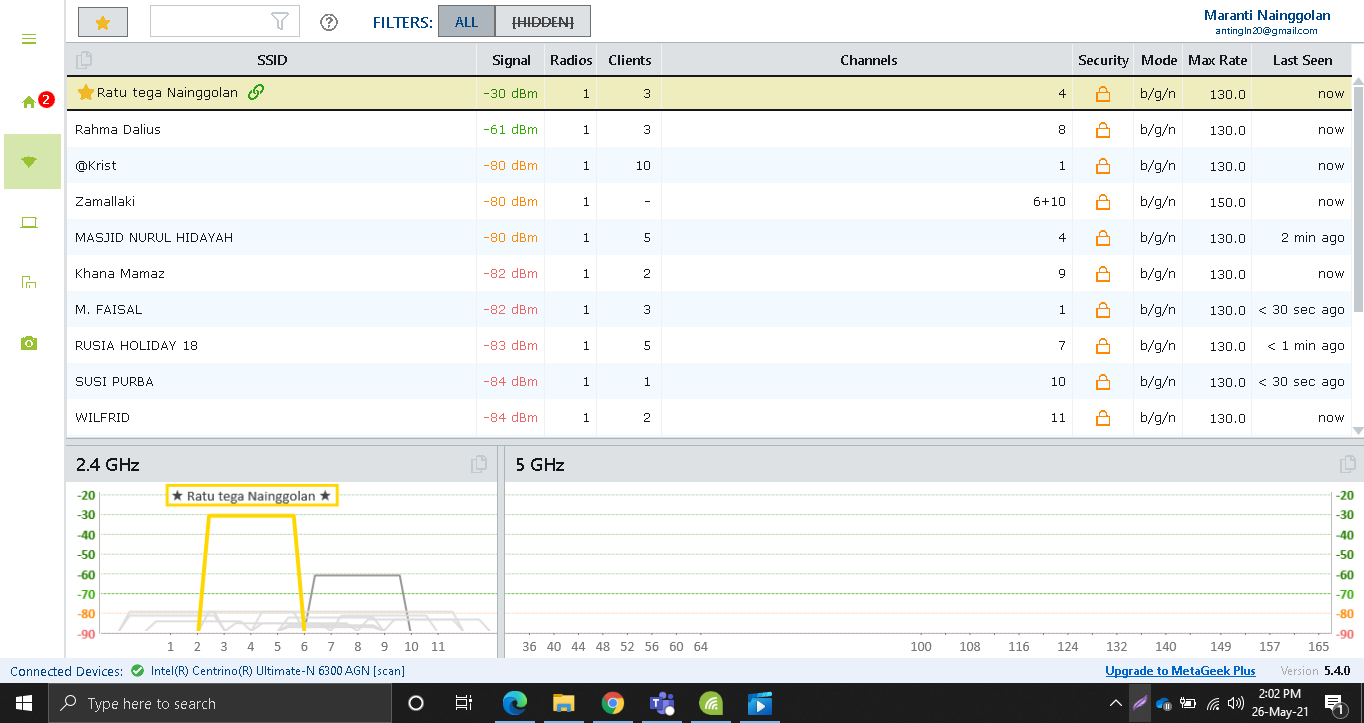
\includegraphics[width=0.4\textwidth]{8.png}
        \caption{Tampilan inSSIDer dalam Rumah}
    \end{figure}

    \begin{figure}
        \centering
        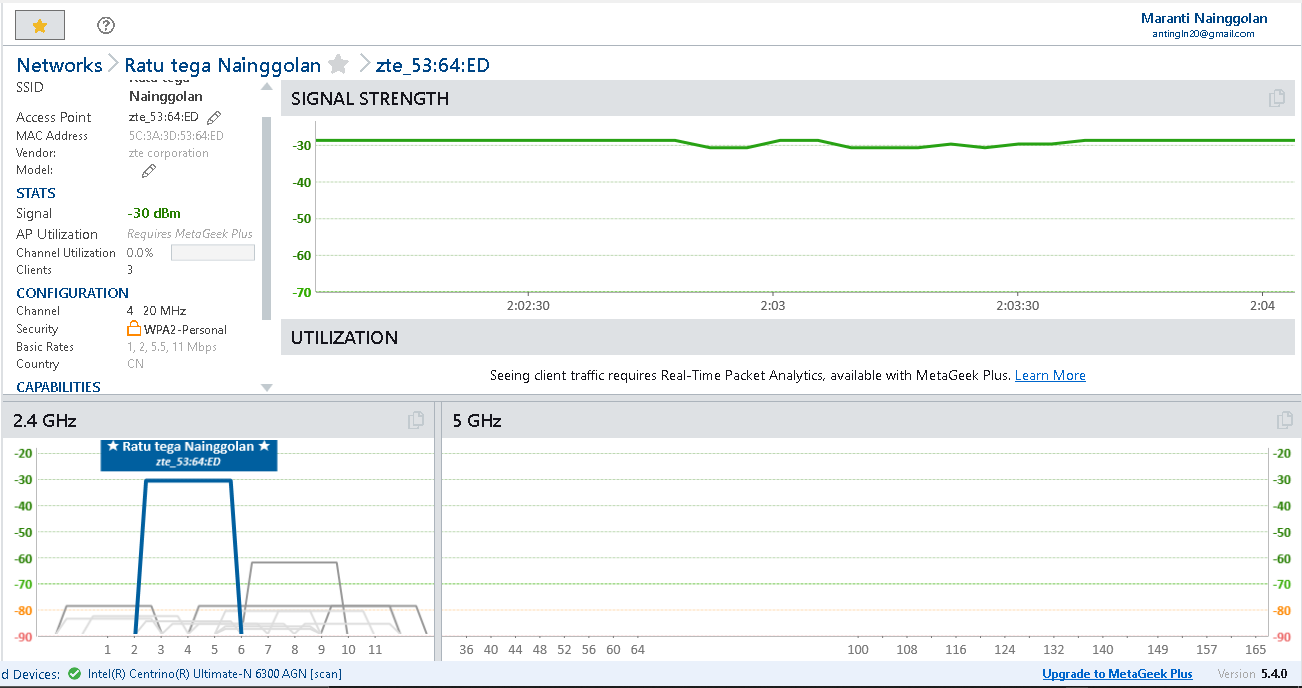
\includegraphics[width=0.4\textwidth]{9.png}
        \caption{Tampilan inSSIDer dalam rumah}
    \end{figure}

\vspace{0.2cm}

Dari AP yang sinyalnya diterima dan tekdeteksi pada inSSIDer terlihat bahwa AP dengan SSID 
"Ratu tega nainggolan" memiliki RSSI (Received Signal Strenght Indicator) yaitu -30 dBm. 
Seting kanal yang digunakan adalah kanal 1 dan bekerja pada frekuensi 2,4 GHz. 
Menggunakan model WPA-2 personal security, 3 client dan memiliki channel 4.
\vspace{0.2cm}

    \item Pengambilan Data dengan Jarak 15 M dari Rumah

    \begin{figure}
        \centering
        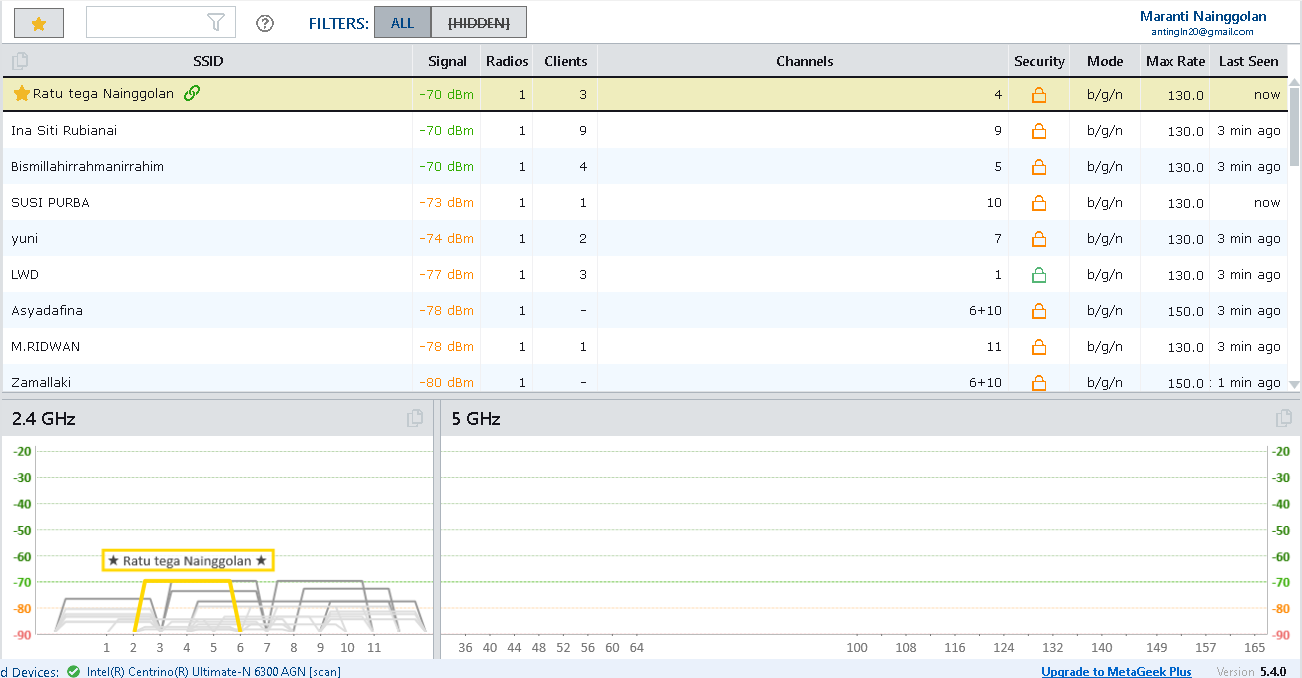
\includegraphics[width=0.4\textwidth]{10.png}
        \caption{Tampilan inSSDer dengan jarak 15 M dari Rumah}
    \end{figure}

    \begin{figure}
        \centering
        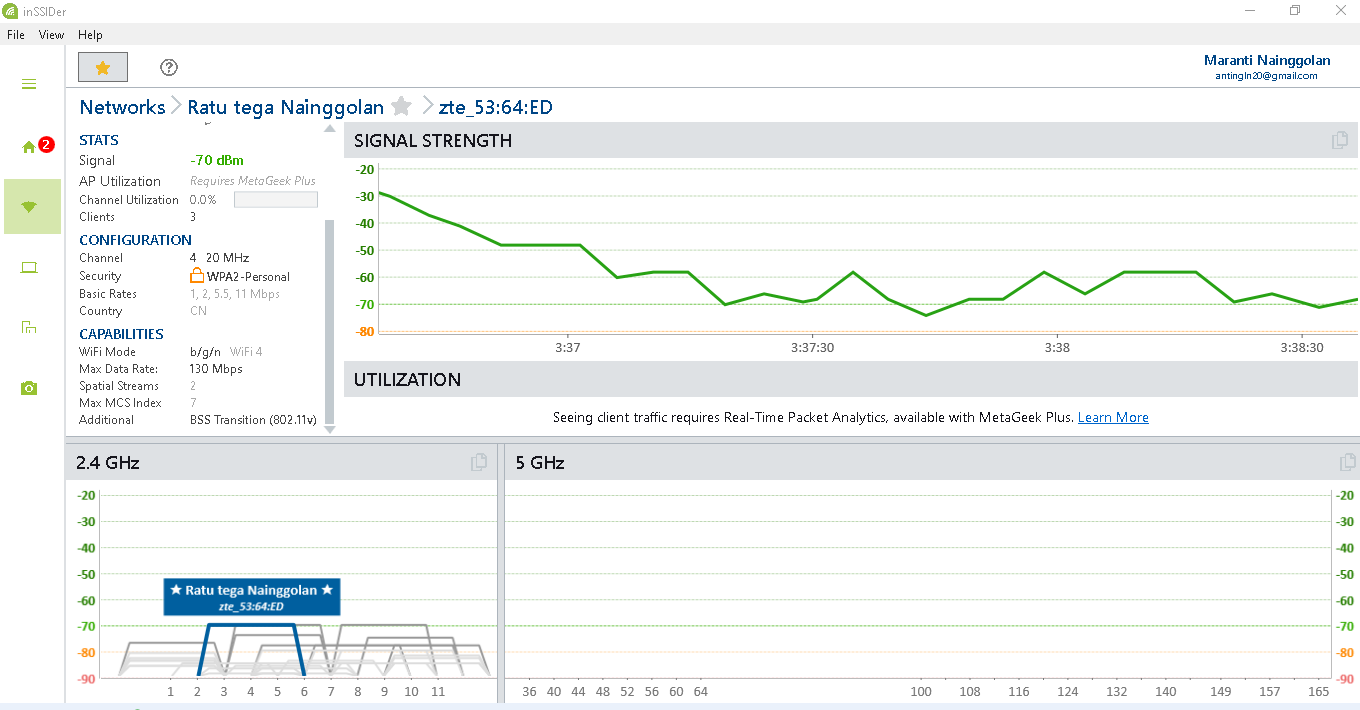
\includegraphics[width=0.4\textwidth]{11.png}
        \caption{Tampilan inSSIDer dengan jarak 15 M dari rumah}
    \end{figure}

\vspace{0.2cm}

Pada gambar diatas terlihat bahwa sinyal wireless dengan
SSID ‘Ratu Tega Nainggolan’ memiliki RSSI (Received
Signal Strength Indicator) yakni -70 dBm. Berada
pada kanal 1 dan bekerja pada frekuensi 2,4 GHz. Menggunakan
model WPA-2 personal security dan memiliki
channel 4
\vspace{0.2cm}  

    \item Pengambilan Data dengan Adanya Penghalang / Pembatas (Dinding)

    \begin{figure}
        \centering
        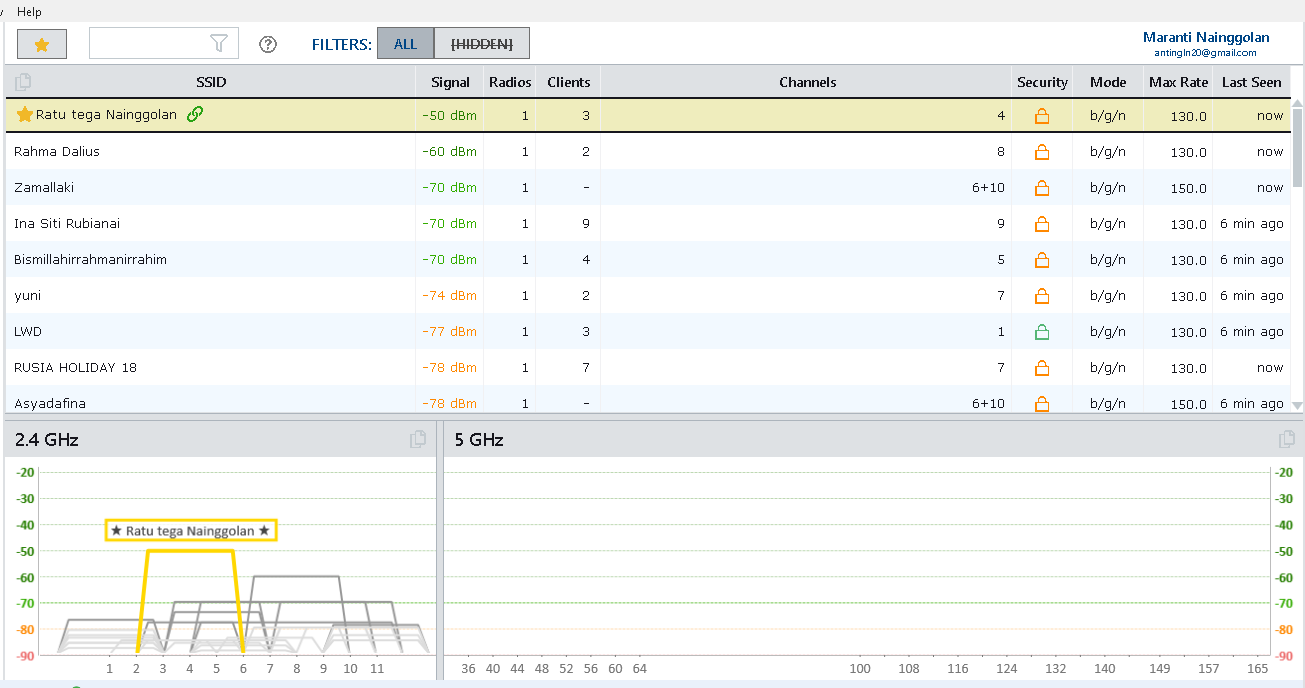
\includegraphics[width=0.4\textwidth]{12.png}
        \caption{Tampilan inSSDer dengan Adanya Pembatas}
    \end{figure}

    \begin{figure}
        \centering
        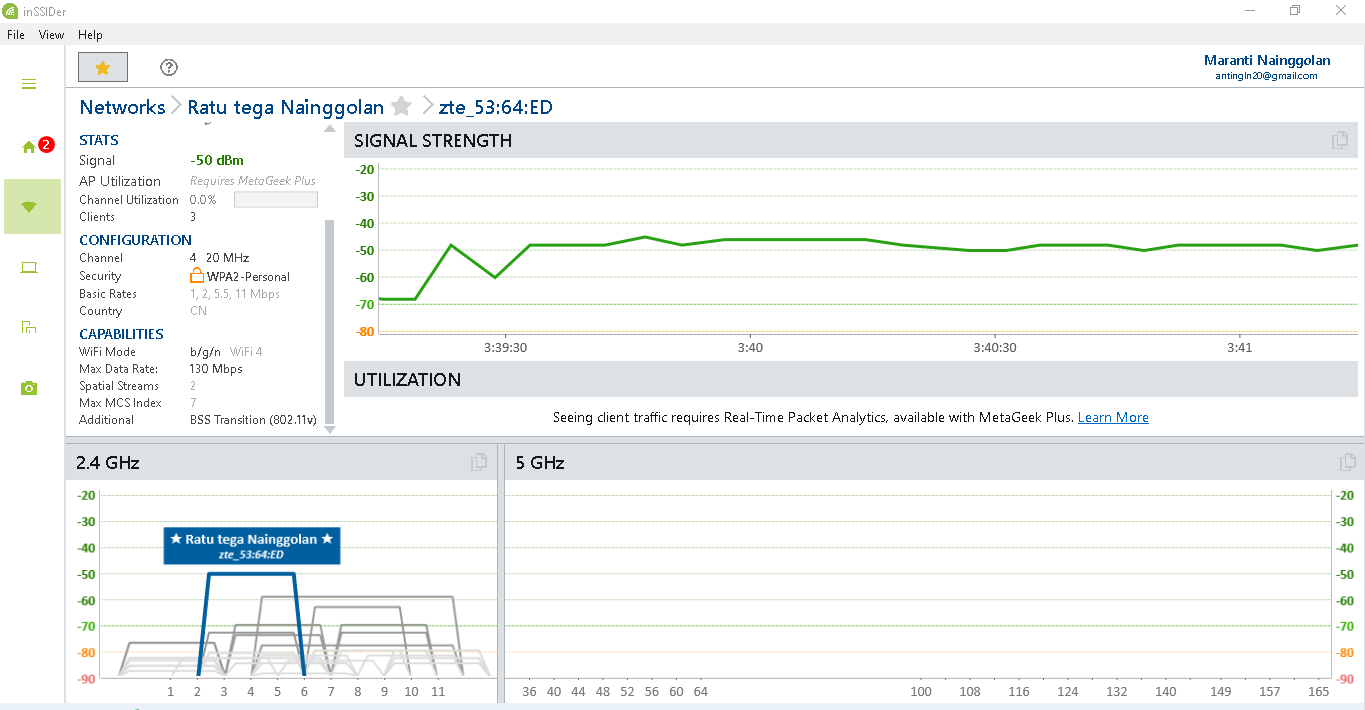
\includegraphics[width=0.4\textwidth]{13.png}
        \caption{Tampilan inSSIDer dengan Adanya pembatas}
    \end{figure}

\vspace{0.2cm}

Pada gambar 8 dan 9 terlihat bahwa sinyal wireless
dengan SSID ‘Ratu Tega Nainggolan’ memiliki RSSI (Received Signal Strength Indicator) yakni -50 dBm.
Berada pada kanal 1 dan bekerja pada frekuensi 2,4
GHz. Menggunakan model WPA-2 personal security dan
memiliki channel 4.
\vspace{0.2cm}

    \item Pengambilan Data Saat Berjalan / Mengelilingi Daerah
    Sekitar

\vspace{0.2cm}

Dalam pengambilan kekuatan sinyal wifi saat berjalan,
tentu kekuatan sinyal nya selalu berubah ubah, itu
dikarenan jarak antara pusat wifi dan tempat pengambilan
data, semakin jauh jarak yg ditelusuri maka kekuatan
siyalnya akan terus melemah, begitupun sebaliknya.
\end{enumerate}

\vspace{0.2cm}
Dari semua gambar diatas dapat dilihat semua AP menggunakan
atau bekerja di frekuensi 2.4 GHz. Frekuensi
ini memang sering digunakan karena merupakan masuk
dalam standard wireless 802.11b dan 802.11g.Sedangkan
Pada data frekuensi 5 GHz tidak ada AP yang
menggunakannya Terlihat pada panel 5GHz capture
tidak ada SSID yang masuk kategori tersebut.Frekuensi
5GHz ini biasanya digunakan pada 802.11a yang notabennya
memiliki max rate yang sama dengan 802.11g
namun dengan pita yang lebih lebar.


\begin{equation}
    Rerata RSSI = \frac{Total Jumlah Nilai RSSI}{Jumlah Koordinat receiver}
    \label{rerata_rssi}
\end{equation}

berdasarkan persamaan~\ref{rerata_rssi}

\section{Kesimpulan}
Pengambilan data untuk mengetahui kekuatan sinyal Wi-
Fi dengan menggunakan inSSIDer telah dilakukan dengan
baik. Dari semua gambar diatas dapat dilihat semua AP
menggunakan atau bekerja di frekuensi 2.4 GHz. Frekuensi ini
memang sering digunakan karena masuk dalam standard wireless
802.11b dan 802.11g. Sedangkan Pada data frekuensi 5 GHz tidak ada AP yang menggunakannya Terlihat pada panel
5GHz capture tidak ada SSID yang masuk kategori tersebut.
Frekuensi 5GHz ini biasanya digunakan pada 802.11a yang
notabennya memiliki max rate yang sama dengan 802.11g
namun dengan pita yang lebih lebar.


\begin{thebibliography}{00}
    \bibitem{b1} IEEE. 802.15.4., Standard 2006, Part 15.4: “Wireless Medium Access Control (MAC) and Physical Layer (PHY) Specifications for Low Rate Wireless
    Personal area Networks (LR WPANs)”, IEEE –SA Standards Board 2006W.-K. Chen, Linear Networks and Systems (Book style). Belmont, CA: Wadsworth,
    1993, pp. 123– 135
    \bibitem{b2} Pranjal., 2013, Experimental Study of a Wireless Local Area Network, International Journal of Information and Computation Technology, Vol.3 No. 10, pp.1047-1052
    \bibitem{b3} Julia Cynthia Rante, Max Alexander Rura Patras. Analisis Kekuatan Sinyal Vol. 14, No. 1, April 2018: 97-102 ISSN: 1907-0837
    \bibitem{b4} Eka, putra, daniel. 2013. Pengamatan Kuat Sinyal Access Point (AP) Menggunakan inSSIDer
    \bibitem{b5} Kapgate, Y., Vatti, R., Jadhav, S., 2017, WiFi Tools and Signal Strength Analysis, GRD Journals Global Research and Development Journal for Engineering , Vol.2 Issue 10.
\end{thebibliography}

\end{document}